\chapter{Trabajos Relacionados}
\section{Consideraciones Iniciales}
En este capítulo se discute... 
\section{Minería Visual de Datos}

Cuando se hace análisis de datos primero se especifica ciertos parámetros para restringir el espacio de búsqueda; de esta forma la minería de datos trabaja de forma automática siguiendo un algoritmo (matemático, estadístico o de inteligencia artificial), finalmente los patrones son encontrados por este algoritmo para luego ser presentados como resultados en pantalla. Dado que existe gran cantidad de patrones generados por el algoritmo de minería de datos automática en forma textual, es casi imposible para el ser humano interpretar y evaluar el patrón en detalle para extraer conocimientos interesantes y características generales. Por otra parte la visualización de información es un estudio de representaciones (interactivas) visuales de datos para reforzar la cognición humana. Estas dos estrategias de de tratamiento de información (minería de datos y visualización de información) pueden llegar a ser complementarias y coexistir en la búsqueda de soluciones para la interpretación de un conjunto de datos complejos o naturales. Por lo tanto, para que la minería de datos sea efectiva es importante incluir a los humanos en el proceso de exploración de datos y combinar la flexibilidad, creatividad y el conocimiento general de la persona con la gran capacidad de almacenamiento y procesamiento de las computadoras de hoy en día. Tal área es denominada \textit{Minería Visual de Datos} \cite{wong1999guest}.

La minería visual de datos tiene como objetivo la integración del humano en el proceso de minería de datos, y la aplicación de las capacidades perceptivas de los humanos para el análisis de grandes conjuntos disponibles. la presentación de los datos en un formulario gráfico en interactivo a menudo fomenta la formación y la validación de nuevas hipótesis, para una buena toma de decisiones por consiguiente una buena resolución de los problemas. Con la visualización obtenemos una la formación y visión de estas hipótesis, la verificación de estas hipótesis se puede realizar también mediante la vía de visualización, pero lo mas conveniente es que vaya respaldado con algunas técnicas automáticas de análisis matemático, estadístico o aprendizaje maquina. 

Ankerst \cite{ankerst2001visual} clasifica en tres enfoques comunes la integración del humano en el proceso de exploración de datos como se muestra en la figura \ref{fig:VDM} :
\begin{itemize}
	\item \textbf{Visualización Anterior.} La visualización de información se realiza antes de que el algoritmo de minería de datos sea ejecutado, con la interacción se tiene un control total sobre el espacio de búsqueda. 
	\item \textbf{Visualización Posterior.} El algoritmo de minería de datos automática se ejecuta primero para la extracción de patrones y estos son mostrados por la visualización, se puede hacer re-calibraciones para posteriores exploraciones, esto con el objetivo de introducir otros parámetros y obtener mejores resultados.
	\item \textbf{Visualización fuertemente Integrado.} Un algoritmo de minería de datos automática realiza un análisis de los datos, pero no produce los resultados finales. Una técnica de visualización se utiliza para presentar los resultados  del proceso de exploración de datos. La combinación de algunos algoritmos de minería de datos automáticos y técnicas de visualización permite  realizar una retroalimentación en el proceso de exploración. De esta forma se permite al usuario entender y llevar mejor el proceso de exploración; trabajar con datos con alto contenido de ruido; no se necesita de alto conocimiento de los algoritmos matemáticos o estadísticos; permite una visión cualitativa de los datos para su posterior análisis cuantitativo.
\end{itemize}

En resumen la minería visual de datos se compone por un lado la minería de datos que son la generación o descubriendo de patrones a partir de un conjunto de datos basándose en técnicas matemáticas, estadísticas o de inteligencia artificial y por otro lado las técnicas de visualización que son la generación de imágenes o de representaciones gráficas a partir de estos datos.
\begin{figure}[!h]
\centering
\includegraphics[width=\columnwidth]{figs/VDM}%
\caption{Vista general de los diferentes enfoques de la integración de los humanos en el proceso de exploración de datos.}%
\label{fig:VDM}%
\end{figure}

\section{Visualización de Información}
La visualización de información \cite{card1999readings} es el uso de representaciones visuales e interactivas de datos para amplificar la cognición. Esto significa que los datos son transformados a una imagen. La imagen puede ser cambiado por los usuarios a medida que se vaya trabajando con él. Esta interacción es importante, ya que permite una constante redefinición de objetivos cuando una nueva visión de los datos se ha obtenido.
Esta área esta ampliando su espectro debido al desarrollo de la visualización en computadoras en tiempo real. Este medio es promisorio porque acrecienta los recursos del humano en la forma de procesamiento perceptual, permite reducir el tiempo de búsqueda de información, permite mejorar el reconocimiento de patrones, permite el uso de  inferencia y monitoreo perceptual en un medio manipulable e interactivo.
Dentro de las subáreas fundamentales se encuentran la visualización de datos multidimensionales, el cual estudiaremos por la importancia dentro del desarrollo del presente trabajo.
\section{Visualización de Datos Multidimensionales}
		\subsection{Proyecciones Multidimensionales}
		\begin{defn}
		 Sea un conjunto de datos $X=\{x_1,x_2,...,x_n\}$ en $\Re^D$ con una función $\delta:\Re^D$X$\Re^D \to \Re$ de disimilaridad entre dos puntos en $\Re^D$ y sea $Y=\{y_1,y_2,...,y_n\}$ un conjunto de datos en $\Re^d$ con $d=\{1,2,3\}$  y $\sigma:\Re^d$X$\Re^d \to \Re$ una función de distancia euclidiana entre dos puntos proyectados en el espacio $\Re^d$. Una proyección multidimensional puede ser descrita con la función inyectiva $f:X \to Y$ que busca hacer de $|\delta(x_i,x_j)-\sigma(f(x_i),f(x_j))|$ más próximo  a cero tanto como sea posible, $ \forall x_i,x_j \in X$.\end{defn} 
\begin{figure}[!h]
\centering
\includegraphics[width=0.6\columnwidth]{figs/PM.pdf}%
\caption{Ejemplo, proyección de datos a un espacio visual 2D.}%
\label{fig:PM}%
\end{figure}
De esta forma, las proyecciones multidimensionales buscan mapear datos definidos en un espacio $\Re^D$(generalmente de alta dimensión $D\geq 4$) en un espacio $\Re^d$ cuya dimensión es menor, $d  \in \{1,2,3\}$, figura \ref{fig:PM}, en la medida de lo posible preservando las distancias entre los vecinos. Esta representación gráfica (posicionamiento de los puntos proyectados) refleja la estructura del conjunto de datos en términos de agrupamiento entre las instancias y otras relaciones de proximidad de interés. Así los puntos preservan una semejanza en relación a la medida de similaridad $\delta$.

El objetivo de reducir la dimensión de los datos puede ser variado dependiendo la aplicación que se busca. En algunos casos se usa la proyección para comprimir una gran base de datos en una cantidad inferior de vectores  representativos \cite{Kohonen2001SM} y algoritmos como \ac{LDA} utilizan la información de la clase a la que cada dato pertenece para realizar la proyección maximizando la definición y las distancias entre distintas clases. 

\subsection{Clasificación}
Con base en la literatura, los métodos de proyección multidimensional pueden ser clasificados de tres formas, Cada una en un contexto  definido diferente. \textcolor[rgb]{0.2,0.8,0.2}{[DESARROLLAR LA CLASIFICACION]}

\subsection{Métricas de medición de calidad de una proyección}
Cuando se trata de medir la calidad de una proyección no existe una forma estándar, como consecuencia en algunos casos la calidad de la proyección queda en manos del criterio del observador. La mayoría de estos métodos se basan en la optimización de algún funcional. En este sentido se han desarrollado varias medidas que buscan establecer que tan bien se preserva la topología del espacio original sobre el espacio visual proyectado. En esta tesis sen presentan cuatro diferentes medidas, el primero (Preservación Topológica) mide la preservación de la estructura de los datos en el espacio proyectado y el segundo (Índice de Dunn) mide la calidad de la compactación y separación de un conjunto de clusters.

\textbf{Preservación Topológica}. La preservación topológica \cite{konig2000interactive} se basa en la comparación de los rankings de vecindad en el espacio original y el espacio visual. Denotamos con $NN_{ji}(i\in[1,k], j\in[1,m])$ y
$nn_{ji}(i\in[1,k], j\in[1,m])$ los $k$ vectores más cercanos a cada vector $j$ en el espacio original y en el espacio proyectado respectivamente. En base a estos rankings a cada dato se le asigna un puntaje de acuerdo a la siguiente regla, donde el parámetro $k$ y $s$ definen la vecindad en torno a cada ejemplo:
 \begin{equation}
	r_{j}=\left\{
                \begin{array}{ll}
									3,~if~NN_{ji} = nn_{ji}\\
									2,~if~NN_{ji} = nn_{jl}, l\in[1,k],i\neq l\\
									1,~if~NN_{ji} = nn_{jt}, t\in[k,s],k<s\\
									0,~\textit{otherwise}
                \end{array}\right.
		\end{equation}
La preservación topológica global se calcula de de la siguiente forma:
\begin{equation}
r=\frac{1}{3mk}\sum^{m}_{j=1}r_j
\end{equation}  		
El valor $r \in [0,1]$ donde  $r=1$ significa una perfecta preservación topológica.

\textbf{Índice de Dunn $(Du)$}. El índice de Dunn \cite{xu2009clustering} es una medida en clusterización que sirve para medir cuan compactos y separados son un conjunto de clusters. $(Du)$ se define como:
\begin{equation}
Du(K)=\min_{i=1,\ldots,K}\left(\min_{j=i+1,\ldots,K}\left(\frac{D(C_i,C_j)}{\max_{l=1,\ldots,K}diam(C_l)}\right)\right)
\end{equation} 
Donde $K$ es el número de clases, $diam(C_i)=\max_{x,y\in C_i}Distancia(x,y)$ es el diámetro del cluster y $D(C_i,C_j)=\min_{x\in C_{i},y\in C_{j}}Distancia(x,y)$ es la distancia entre clusters.
Un valor mayor para el índice $Du(K)$ implica clusters más separados y bien definidos (compactos). Si bien esta métrica no mide la calidad de la proyección, no mide preservación topológica, sirve para medir la capacidad del método para preservar la separación de los clusters, que puede ser útil y atractivo en algunas aplicaciones. 

\subsection{Técnicas de Visualización Radial}
Utilizamos el termino de visualización radial para describir un sistema interactivo que organiza los datos en forma circular y/o elíptica. La prevalencia de los métodos de visualización radial es debido a su atractivo estético y su facilidad de exploración.

Visualizaciones radiales actuales muestran una notable diversidad en su diseño visual y métodos de interacción. Geoffrey \cite{draper2009survey} propone siete patrones de alto nivel de diseño o arquetipos que describen casi todos los sistemas de visualización radiales basándose en los segmentos de linea desde el punto central y área de ocupación del circulo. Estas características dieron lugar a tres divisiones los cuales se detallan en la tabla \ref{table:vr}: \textbf{\textit{Polar Plot}}, \textbf{\textit{Space Filling}} y \textbf{\textit{Ring}}.

\begin{table}[]
\centering
\begin{tabular}{|c|c|c|}
\hline
                  & Patrones & Ejemplos  \\ \hline
\multirow{2}{*}{Polar Plot} &Tree  & \cite{Jankun:2003:MoireGraphs}, \cite{Lamping:1995:FTB},  \\ \cline{2-3} 
                  & Star  &  \citar{kandogan:2000:starcoordinates}, \cite{havre2001interactive}\\ \hline
\multirow{3}{*}{Space Filling} 
									& Concentric & \cite{cugini1996interactive}, \cite{keim2006monitoring}  \\ \cline{2-3} 
                  & Spiral & \cite{Carlis:1998:IVS}, \cite{dragicevic2002spiraclock} \\ \cline{2-3} 
                  & Euler & \cite{van2003bubbleworld}, \cite{hong2003zoomology} \\ \hline
\multirow{2}{*}{Ring} & Connected & \cite{livnat2005visualization}, \cite{salton1996automatic} \\ \cline{2-3} 
                  & Disconnected & \cite{brewer2000collaborative}, \cite{draper2008votes} \\ \hline
\end{tabular}
\label{table:vr}
\caption{Diseño de patrones para la visualización Radial }
\end{table}

%\textcolor[rgb]{0.2,0.8,0.2}{[TABLA DE TODOS LAS VISUALIZACIONES RADIALES]}
%\begin{table}[]
%\centering
%\begin{tabular}{|c|c|c|}
%\hline
%                  & Patrones & Ejemplos  \\ \hline
%\multirow{2}{*}{Polar Plot} &Tree  & ~\cite{Jankun:2003:MoireGraphs}, ~\cite{Lamping:1995:FTB},  \\ \cline{2-3} 
%                  & Star  &  ~\citar{kandogan:2000:starcoordinates}, ~\cite{havre2001interactive}, ~\cite{spence2001information}\\ \hline
%\multirow{3}{*}{Space Filling} 
%									& Concentric & \cite{cugini1996interactive}, \cite{keim2006monitoring}, \cite{yang2002interring}  \\ \cline{2-3} 
%                  & Spiral & \cite{Carlis:1998:IVS}, \cite{dragicevic2002spiraclock}, \cite{weber2001visualizing} \\ \cline{2-3} 
%                  & Euler & \cite{van2003bubbleworld}, \cite{hong2003zoomology}, \cite{mohammadi2005moiretrees} \\ \hline
%\multirow{2}{*}{Ring} & Connected & \cite{livnat2005visualization}, \cite{salton1996automatic} \\ \cline{2-3} 
%                  & Disconnected & \cite{brewer2000collaborative}, \cite{draper2008votes}, \cite{suntinger2008event} \\ \hline
%\end{tabular}
%\end{table}


\textbf{\textit{Polar Plot}}.  Patrones Polares son aquellos en los nodos se extienden radialmente desde el centro de la circunferencia pero no necesariamente tienen la misma longitud, esta longitud tiene algún significado semántico. \textit{Polar Plot} esta dividido en dos campos \textbf{Tree} (visualización y exploración de estructuras de datos jerárquicas como arboles) y \textbf{Star} (visualización de las relaciones entre entidades dispares).
\textcolor[rgb]{0.2,0.8,0.2}{[IMAGEN]}
\begin{figure}[!h]
\centering
\includegraphics[width=0.6\columnwidth]{figs/PolarPlot}%
\caption{Polar Plot}%
\label{fig:PolarPlot}%
\end{figure}

\textbf{\textit{Space Filling}}. Son patrones que lo que buscan es cubrir todo el espacio de manera eficiente.  \textit{Space Filling} está dividido en tres campos: \textbf{Concentric} ( anillos concentricos divididos en múltiples sectores, también sirve para la visualización de estructuras de datos jerarquices); \textbf{Spiral} (origen en el centro del canvas, utilizado para la visualización de datos periódicos de serie, tales como datos temporales) y \textbf{Euler} (múltiples círculos ubicados en el interior o cerca a un circulo más grande, puede anidar niveles de profundidad; utilizado para la visualización de datos jerárquicos).
\textcolor[rgb]{0.2,0.8,0.2}{[IMAGEN]}
\begin{figure}[!h]
\centering
\includegraphics[width=0.6\columnwidth]{figs/SpaceFilling}%
\caption{Polar Plot}%
\label{fig:SpaceFilling}%
\end{figure}

\textbf{\textit{Ring}}. Los patrones \textit{ring} combinan \textit{Polar Plot} y \textit{Space Filling}. Los nodos de interés son colocados alrededor de la circunferencia de un anillo y la información adicional puede aparecer dentro del anillo. \textit{Ring} se divide en 2 campos \textbf{Connected} (Nodos posicionados alrededor del circulo y estos están unidos por segmentos de lineas; utilizados para visualizar la relación entre entidades disparejas) y \textbf{Disconnected} (nodos posicionados alrededor de una circunferencia, algunos datos se encuentran dentro de la circunferencia, utilizado para la visualización la relación entre los datos).
\textcolor[rgb]{0.2,0.8,0.2}{[IMAGEN]}
\begin{figure}[!h]
\centering
\includegraphics[width=0.6\columnwidth]{figs/Ring}%
\caption{Polar Plot}%
\label{fig:Ring}%
\end{figure}

\subsection{Radviz \textcolor[rgb]{0.2,0.8,0.2}{[PONER IMAGEN]}} 
Radviz \cite{hoffman1997radviz} es una técnica de visualización radial que puede mostrar datos multidimensionales sobre una proyección bi-dimensional. Los atributos de estos datos se presentan como puntos de anclaje equidistantes a lo largo del perímetro del circulo que tiene como radio la unidad. Las instancias de datos se representan por medio de puntos y se muestran dentro del circulo, sus posiciones están determinadas por una matadora de la física: cada punto se mantiene en su lugar con los resortes que se ajustan en el otro extremo a los anclajes de los atributos, la rigidez de estos resortes dependen del valor que tienen para cada atributo. Naturalmente estos datos deben tener valores entre 0 y 1 para todos los atributos. 
\begin{defn} 
Sea un conjunto de datos $X=\{x_1,x_2,\ldots,x_n\}$ en $\Re^D$, y el vector $V=\{v_1,v_2,\ldots,v_D\}$ que contiene las posiciones de los atributos de anclaje, la representación en baja dimensión $y_{j}$ de un dato $j$ esta dado por la siguiente ecuación:
\end{defn}
\begin{equation}
y_{j}=\frac{\sum_{i}^{D}{x_{ji}v_{i}}}{\sum_{i}^{D}{x_{i}}}
\end{equation}
Desde la primera versión de Radviz se propusieron algunas variantes con el fin de mejorar algunas capacidades. Sharko propuso \ac{VRV} \cite{sharko2008vrv} con el objetivo de extender la abilidad de Radviz para que pueda visualizar conjuntos de datos complejos. La idea radica en incrementar el número de puntos de anclaje utilizando información de los datos, por ejemplo cuando se trata de atributos categóricos se aumenta tantos puntos de anclaje como valores posibles tenga el atributo, de esta forma se busca una mejor re-ubicación de los puntos. Russell \cite{russell2012voronoi_radviz} propone una variación en el que se combina Radviz con particionamiento basado en voronoi esto con el objetivo de mejorar la calidad  y la formación de los clusters en la proyección. Ono propuso \textit{Concentric RadViz} \cite{ono2015cradviz} con la finalidad de visualizar datos que tienen cierta ambigüedad en su clasificación (datos multi-clase).

Naturalmente Radviz tiene ciertos inconvenientes como la sobreposición de los datos y la poca facilidad de exploración cuando se trata de conjunto de datos de muy alta dimensión, como se muestra en la figura \textcolor[rgb]{0.2,0.8,0.2}{[REFERENCIAR FIGURA].}
\subsection{Star Coordinates} 
Star Coordinates \cite{kandogan:2000:starcoordinates} al igual que Radviz busca visualizar datos en alta dimensión sobre una proyección bi-dimensional. Los atributos son posicionados en forma de ejes de coordenadas con con un origen en común, con igual longitud e igual angulo entre ellos (inicialmente). Los datos posicionan dependiendo de una combinación lineal del valor que tiene para cada atributo con las longitudes y direcciones de los ejes (los cuales influyen directamente en la posición final del dato). 

\begin{defn} 
Sea un conjunto de datos $X=\{x_1,x_2,\ldots,x_n\}$ en $\Re^D$, y el vector $V=\{v_1,v_2,\ldots,v_D\}$ que contiene las posiciones de los extremos de los ejes, la representación en baja dimensión $y_{j}$ de un dato $j$ esta dado por la siguiente ecuación:
\end{defn}
\begin{equation}
y_{j}=x_{j1}\vec{v}_1 + x_{j2}\vec{v}_2 + \ldots + x_{jD}\vec{v}_D= \sum^{D}_{i=1}{x_{ji}\vec{v}_j}
\end{equation}}
Star Coordinates cuenta con algunas variantes de los cuales se menciona solo algunas: Lehmann propuso \textit{Orthographic Star Coordinates} \cite{lehmann:2013:osc} con el objetivo de eliminar las distorsiones de la proyección, la idea radica en la formulación de las condiciones de los ejes de coordenados para definir proyecciones ortográficas, mediante la optimización no lineal repetida en cada modificación. Yang Sun propuso una técnica \cite{yang:2008:scMultivariate} variante del Star Coordinates con el objetivo de superar ciertos inconvenientes de la proyección original, inconvenientes como la dificultad de configuración manual de los ejes, esto basándose en calibraciones en los ángulos de los ejes.

Star Coordinates cuenta con 2 operaciones interactivas: \textbf{Escala} que consiste en cambiar la longitud del eje, de esta forma se aumenta o disminuye la contribución del eje sobre la proyección final y \textbf{Rotación} que consiste en cambiar la dirección del eje, al cambiar la dirección del eje también se cambia la dirección de esta sobre la proyección final. 
Al igual que Radviz, Star Coordinates tiene ciertos inconvenientes cuando se manejan datos de muy alta dimensión, específicamente este inconveniente radica en que no se tiene control de los atributos que se explora, como se muestra en la figura \textcolor[rgb]{0.2,0.8,0.2}{[REFERENCIAR]}

\section{Consideraciones Finales}
